The background chapter will outline the considerations that needs to be made when testing the usability of sensory feedback configurations in combination with myoelectric prosthetic control. The feedback will be given based on which motion state a pattern recognition controlled prosthesis is in. \\ 
The main idea behind myoelectric prosthetic control is to translate recorded muscle signals (EMG signals) into a motion performed by the prosthesis. A pattern recognition model can be taught to differentiate between a set of movement classes. When receiving a segmented part of a EMG signal it then decides upon which movement class that most likely is being performed. In combination with the elicited muscle contraction level, this is used as input in the control system and the prosthesis should perform a corresponding motion. In a closed loop prosthesis, the motion state the prosthesis is in can be coded to be equivalent to a certain sensory feedback. The should enable the user to interpret the sensory feedback and use as additional information to visual feedback about the prosthesis' state. A closed loop prosthesis iteration can be seen in \figref{fig:closed_loop_pros}. \\
Regarding control the background chapter will explain the following: generation of EMG signals, data acquisition, data processing, pattern recognition and proportional control. Regarding sensory feedback the following will be explained: prior investigations on sensory feedback, types of sensory feedback and sensory feedback configurations. 

\begin{figure}[H]                 
	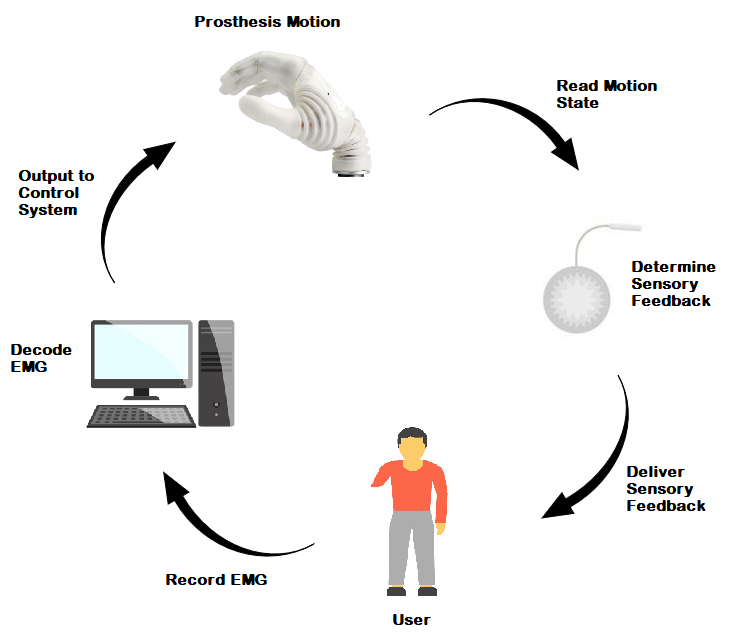
\includegraphics[width=.65\textwidth]{figures/closed_loop_pros}  
	\caption{The figure shows the stages of a closed loop prosthesis. First, EMG signals are recorded from the user. The signals are decoded and an output is relayed to the control system, which is used for the prosthesis to perform a motion. The motion state is then read and sensory feedback is delivered to the user regarding which motion state the prosthesis is in.}
	\label{fig:closed_loop_pros} 
\end{figure}